\documentclass[hyperref, a4paper]{article}

\usepackage{geometry}
\usepackage{titling}
\usepackage{titlesec}
\usepackage{booktabs}
\usepackage{multirow}
\usepackage{enumitem}
\usepackage{footnote}
\usepackage{enumerate}
\usepackage{amsmath, amssymb, amsthm}
\usepackage{mathtools}
\usepackage{bbm}
\usepackage{cite}
\usepackage{graphicx}
\usepackage{subfigure}
\usepackage{physics}
\usepackage{tensor}
\usepackage{siunitx}
\usepackage[version=4]{mhchem}
\usepackage{tikz}
\usepackage{xcolor}
\usepackage{listings}
\usepackage{autobreak}
\usepackage[ruled, vlined, linesnumbered]{algorithm2e}
\usepackage{nameref,zref-xr}
\zxrsetup{toltxlabel}
\usepackage[colorlinks,unicode]{hyperref} % , linkcolor=black, anchorcolor=black, citecolor=black, urlcolor=black, filecolor=black
\usepackage[most]{tcolorbox}
\usepackage{prettyref}

% Page style
\geometry{left=3.18cm,right=3.18cm,top=2.54cm,bottom=2.54cm}
\titlespacing{\paragraph}{0pt}{1pt}{10pt}[20pt]
\setlength{\droptitle}{-5em}

% More compact lists 
\setlist[itemize]{
    itemindent=17pt, 
    leftmargin=1pt,
    listparindent=\parindent,
    parsep=0pt,
}

% Math operators
\DeclareMathOperator{\timeorder}{\mathcal{T}}
\DeclareMathOperator{\diag}{diag}
\DeclareMathOperator{\legpoly}{P}
\DeclareMathOperator{\primevalue}{P}
\DeclareMathOperator{\sgn}{sgn}
\DeclareMathOperator{\res}{Res}
\newcommand*{\ii}{\mathrm{i}}
\newcommand*{\ee}{\mathrm{e}}
\newcommand*{\const}{\mathrm{const}}
\newcommand*{\suchthat}{\quad \text{s.t.} \quad}
\newcommand*{\argmin}{\arg\min}
\newcommand*{\argmax}{\arg\max}
\newcommand*{\normalorder}[1]{: #1 :}
\newcommand*{\pair}[1]{\langle #1 \rangle}
\newcommand*{\fd}[1]{\mathcal{D} #1}
\DeclareMathOperator{\bigO}{\mathcal{O}}

% TikZ setting
\usetikzlibrary{arrows,shapes,positioning}
\usetikzlibrary{arrows.meta}
\usetikzlibrary{decorations.markings}
\tikzstyle arrowstyle=[scale=1]
\tikzstyle directed=[postaction={decorate,decoration={markings,
    mark=at position .5 with {\arrow[arrowstyle]{stealth}}}}]
\tikzstyle ray=[directed, thick]
\tikzstyle dot=[anchor=base,fill,circle,inner sep=1pt]

% Algorithm setting
% Julia-style code
\SetKwIF{If}{ElseIf}{Else}{if}{}{elseif}{else}{end}
\SetKwFor{For}{for}{}{end}
\SetKwFor{While}{while}{}{end}
\SetKwProg{Function}{function}{}{end}
\SetArgSty{textnormal}

\newcommand*{\concept}[1]{{\textbf{#1}}}

% Embedded codes
\lstset{basicstyle=\ttfamily,
  showstringspaces=false,
  commentstyle=\color{gray},
  keywordstyle=\color{blue}
}

% Reference formatting
\newrefformat{fig}{Figure~\ref{#1}}
\newrefformat{tbl}{Table~\ref{#1}}

% Color boxes
\tcbuselibrary{skins, breakable, theorems}
\newtcbtheorem[number within=section]{warning}{Warning}%
  {colback=orange!5,colframe=orange!65,fonttitle=\bfseries, breakable}{warn}
\newtcbtheorem[number within=section]{note}{Note}%
  {colback=green!5,colframe=green!65,fonttitle=\bfseries, breakable}{note}
\newtcbtheorem[number within=section]{info}{Info}%
  {colback=blue!5,colframe=blue!65,fonttitle=\bfseries, breakable}{info}

\newenvironment{shelldisplay}{\begin{lstlisting}}{\end{lstlisting}}

\title{Homework 4}
\author{Jinyuan Wu}

\begin{document}

\maketitle

\paragraph{Exercise 3 in lecture 12}

\paragraph{Solution} The normalization factor in the time domain is 
\begin{equation}
    \int_{-\infty}^\infty \abs{g(t)}^2 \dd{t} = \sigma \sqrt{\pi}.
\end{equation}
The expectation values are 
\begin{equation}
    \expval{t^2} = \frac{\int_{-\infty}^\infty \dd{t} \abs{g(t)}^2 t^2 }{\int_{-\infty}^\infty \dd{t} \abs{g(t)}^2}
    = t_0^2 + \frac{1}{2} \sigma^2,
\end{equation}
and 
\begin{equation}
    \expval{t} = \frac{\int_{-\infty}^\infty \dd{t} \abs{g(t)}^2 t }{\int_{-\infty}^\infty \dd{t} \abs{g(t)}^2}
    = t_0.
\end{equation}
The frequency domain version of $g$ is 
\begin{equation}
    g[\omega] = \int_{-\infty}^\infty \ee^{\ii \omega t} g(t) 
    = \sigma \sqrt{2\pi} \ee^{\ii (\omega - \omega_0) t - \frac{1}{2} \sigma^2 (\omega - \omega_0)^2}.
\end{equation}
The normalization factor is 
\begin{equation}
    \int_{-\infty}^\infty \abs{g[\omega]}^2 \dd{\omega} 
    = 2 \pi \sigma^2 \cdot \sqrt{\frac{\pi}{\sigma^2}} = 2 \pi^{3/2} \sigma.
\end{equation}
The expectation values are 
\begin{equation}
    \expval{\omega^2} = \frac{
        \int_{-\infty}^\infty \dd{\omega} \abs{g[\omega]}^2 \omega^2
    }{
        \int_{-\infty}^\infty \dd{\omega} \abs{g[\omega]}^2
    } = \frac{1}{2 \sigma^2} + \omega_0^2,
\end{equation}
and 
\begin{equation}
    \expval{\omega} = \omega_0.
\end{equation}
So 
\begin{equation}
    \begin{aligned}
        \sigma_t \sigma_\omega &= 
        \sqrt{ \expval{t^2} - \expval{t}^2 } \sqrt{ \expval{\omega^2} - \expval{\omega}^2 } \\
        &= \sqrt{ \frac{1}{2} \sigma^2 \cdot \frac{1}{2 \sigma^2} } = \frac{1}{2}.
    \end{aligned}
\end{equation}
So indeed for $g(t)$,
$\sigma_t \sigma_\omega$ reaches its minimum value.

\paragraph{Exercise 1 in lecture 13} We have the following transmission model: the sent signal $X$ has 3 possible values $x=0, \pm 1$ with $p_0=p_1=p_{-1}=1 / 3$. The noise $\Xi$ has two possible values $\zeta=\pm 1$. We suppose the channel function $F$ has the following expression $Y=\operatorname{Im}\left[\mathrm{e}^{i 2 \pi(X+\Xi) / }\right]$. What are all the possible values of $Y$ ? Give the expression of the distributions $w(x), w(y), w(x, y)$ and $w(y \mid x)$.

\paragraph{Solution} The possible results are listed in \prettyref{tbl:prob-y}.
The possible values of $Y$ are $0$ and $\pm \sqrt{3}/ 2$.
From \prettyref{tbl:prob-y} we have
\begin{equation}
    w(x) = \begin{cases}
        \frac{1}{3}, \quad x = 0, \\
        \frac{1}{3}, \quad x = 1, \\
        \frac{1}{3}, \quad x = -1,
    \end{cases}
\end{equation}
\begin{equation}
    w(y) = \begin{cases}
        \frac{1}{3}, \quad y = 0, \\
        \frac{1}{3}, \quad y = \sqrt{3} / 2, \\
        \frac{1}{3}, \quad y = - \sqrt{3} / 2,
    \end{cases}
\end{equation}
and 
\begin{equation}
    w(x , y) = \begin{cases}
        \frac{1}{6}, \quad (x, y) = (0, \sqrt{3} /2), \\
        \frac{1}{6}, \quad (x, y) = (0, - \sqrt{3} / 2), \\
        \frac{1}{6}, \quad (x, y) = (1, - \sqrt{3} / 2), \\
        \frac{1}{6}, \quad (x, y) = (1, 0), \\
        \frac{1}{6}, \quad (x, y) = (-1, 0), \\
        \frac{1}{6}, \quad (x, y) = (-1, \sqrt{3}/2), \\
        0, \quad \text{otherwise}.
    \end{cases}
\end{equation}
So 
\begin{equation}
    w(y | x) = \frac{w(x, y)}{w(x)} = 
    \begin{cases}
        \frac{1}{2}, \quad (x, y) = (0, \sqrt{3} /2), \\
        \frac{1}{2}, \quad (x, y) = (0, - \sqrt{3} / 2), \\
        \frac{1}{2}, \quad (x, y) = (1, - \sqrt{3} / 2), \\
        \frac{1}{2}, \quad (x, y) = (1, 0), \\
        \frac{1}{2}, \quad (x, y) = (-1, 0), \\
        \frac{1}{2}, \quad (x, y) = (-1, \sqrt{3}/2), \\
        0, \quad \text{otherwise}.
    \end{cases}
\end{equation}

\begin{table}
    \centering
    \caption{Probabilistic distribution of $Y$; the probability of each row is $1/6$.}
    \label{tbl:prob-y}

    \begin{tabular}{ccc}
    \toprule
    $X$                 & $\Xi$ & $Y = \Im \ee^{\ii 2 \pi(X+\Xi) / 3}$ \\ \midrule
    \multirow{2}{*}{0}  & 1     & $\frac{\sqrt{3}}{2}$                 \\
                        & -1    & $-\frac{\sqrt{3}}{2}$                \\ \midrule
    \multirow{2}{*}{1}  & 1     & $-\frac{\sqrt{3}}{2}$                \\
                        & -1    & $0$                                  \\ \midrule
    \multirow{2}{*}{-1} & 1     & $0$                                  \\
                        & -1    & $\frac{\sqrt{3}}{2}$                 \\ \bottomrule 
    \end{tabular}
\end{table}

\paragraph{Exercise 2 in lecture 14}

\paragraph{Solution} Suppose $p$ is the probability of $X = -1$,
and we have 
\begin{equation}
    m = \expval{X} = - p + (1 - p) = 1 - 2p, \quad -1 \leq m \leq 1,
\end{equation}
and therefore 
\begin{equation}
    p = \frac{1 - m}{2}, 
\end{equation}
and 
\begin{equation}
    \begin{aligned}
        H_\alpha(X) &= \frac{1}{1 - \alpha} \log_2(p^{\alpha} + (1 - p)^\alpha) \\
        &= \frac{1}{1 - \alpha} \log_2\left(
            \left( \frac{1 - m}{2} \right)^{\alpha}
            + \left( \frac{1 + m}{2} \right)^{\alpha}
        \right).
    \end{aligned}
\end{equation}
The plots can be found in \prettyref{fig:entropy-plot}.

\begin{figure}
    \centering
    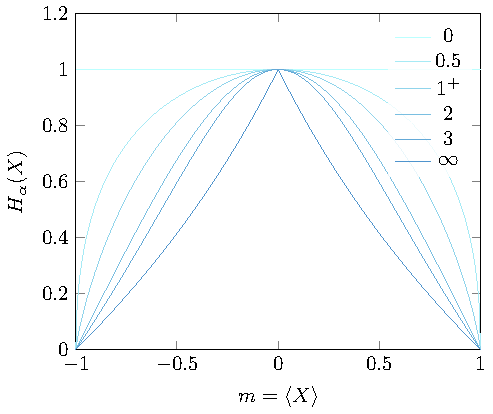
\includegraphics[width=0.7\textwidth]{plots/ising-entroy-alpha.pdf}
    \caption{Plots of $H_\alpha(X)$ with different $\alpha$'s}
    \label{fig:entropy-plot}
\end{figure}



\end{document}